\cchapter{مقدمه}
\section{واقعیت افزوده چیست؟}
در سال ۱۹۷۷ خیلی از علاقه‌مندان به فیلم و سینما، با دیدن تصویر ۳ بعدی از زنی در هوا که در حال گفتن جمله‌ی،  \lr{"Help me Obiwan-Kenobi you’re my only hope"} بود، شگفت‌زده شدند. این صحنه فوق‌العاده متعلق به فیلم \lr{Star Wars} \LTRfootnote{http://www.starwars.com}بود که با استفاده از افکت‌های مخصوص توانسته بودند محتوای ۳ بعدی و مجازی را در دنیای واقعی خلق بکنند. این فیلم صحنه‌ای از آینده را نشان می‌داد که در آن مردم می‌توانستند در دنیایی که اجسام واقعی و مجازی باهم ترکیب‌شده‌اند، به‌راحتی مانند دنیای واقعی با کامپیوترها ارتباط برقرار بکنند.
\\
حدود ۳۰ سال بعد در سال ۲۰۰۸، در میان برگزاری انتخابات ریاست جمهوری آمریکا، یک نمایشِ ویژه از تکنولوژی به مردم نشان داده شد. در میان صحبت در رابطه با انتخابات توسط شبکه \lr{CNN}، خبرنگار \lr{Wolf Blitzer }به سمت جایگاه خالی نگاه کرد و ناگهان خبرنگار \lr{Jessica Yellin } بر روی صحنه به‌صورت ۳ بعدی و درون برنامه زنده ظاهر شد\LTRfootnote{http://edition.cnn.com/2008/TECH/11/06/hologram.yellin/}. \lr{Wolf} قادر بود با او، صحبت کند و یک مکالمه زنده و رودررو داشته باشد درصورتی‌که \lr{Jessica Yellin }  هزاران مایل با او فاصله داشت.
\\
این‌یک مثال از واقعیت افزوده بود \LTRfootnote{Augmented Reality} که به‌اختصار به آن \lr{AR} نیز گفته می‌شود که قادر است تصاویر مجازی را بسازد و به دنیای واقعی اضافه کند. واقعیت افزوده تکنولوژی است که در دسته فنّاوری‌های مرتبط با ارتباط انسان و کامپیوتر \LTRfootnote{human computer interaction technology} قرار می‌گیرد، که در این دسته فنّاوری‌هایی قرار می‌گیرند که باعث برقراری ارتباط  بهتر انسان و کامپیوتر می‌گردند و شروع این تکنولوژی‌ها از حدود دهه ۱۹۶۰ است با به وجود آمدن کارت‌های پانچ شروع شد و در ادامه این روند به موس‌ها، کیبوردها و ... رسید. هدف این تکنولوژی این است که رابط کاربری  کاربران که درک و ارتباط با آن دشوار است را از دید آن‌ها مخفی کند و ارتباط با کامپیوتر را بسیار ساده‌تر مانند ارتباط با دنیای واقعی بکند.
\\
مثال‌های بالا به ما نشان می‌دهد که واقعیت افزوده چقدر در ارتباطات و نمایش اطلاعات می‌تواند به ما کمک بکند و همین‌طور مانند تکنولوژی‌های دیگر، واقعیت افزوده می‌تواند در سطح خیلی گسترده‌تری نیز به‌کار برود. محققین تا به امروز در حوزه‌های مختلفی از این تکنولوژی استفاده کرده‌اند مانند پزشکی، سرگرمی، مهندسی، آموزش نظامی و غیره. برای نمونه در پزشکی می‌توان اطلاعات بیمار را بر روی بدن فرد بیمار به نمایش درآورد \cite{nasir}و در رابطه با سرگرمی، بازیکنان می‌توانند در دنیای واقعی به بازی بپردازند \cite{Piekarski}و یا در مهندسی، مهندسان می‌توانند انتهای یک پروژه ساختمانی را ببینند\cite{Fjeld}.
\\


	\begin{figure}
		\centering
		\begin{subfigure}[b]{0.4\textwidth}
			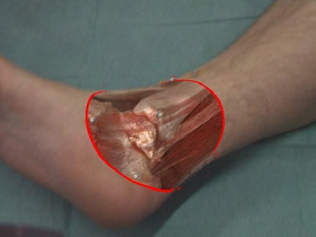
\includegraphics[width=\textwidth]{image/AR_in_medicine}
			\caption{استفاده از واقعیت افزوده در پزشکی
			\\
		\cite{nasir}}
			\label{fig:gull}
		\end{subfigure}
		~ %add desired spacing between images, e. g. ~, \quad, \qquad, \hfill etc. 
		%(or a blank line to force the subfigure onto a new line)
		\begin{subfigure}[b]{0.4\textwidth}
			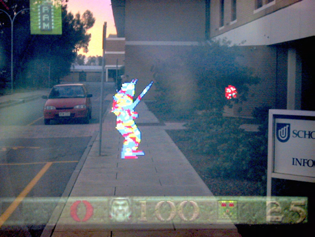
\includegraphics[width=\textwidth]{image/ARQuake_outdoor_AR_game}
			\caption{استفاده از واقعیت افزوده برای بازی
			\\
			\cite{Piekarski}}
			\label{fig:tiger}
		\end{subfigure}
		~ %add desired spacing between images, e. g. ~, \quad, \qquad, \hfill etc. 
		%(or a blank line to force the subfigure onto a new line)
		
		\begin{subfigure}[b]{0.4\textwidth}
			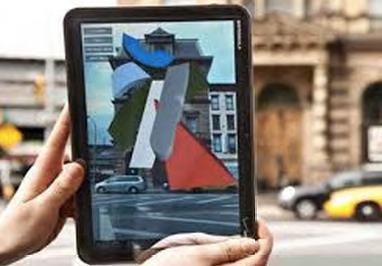
\includegraphics[width=\textwidth]{image/AR_architecture_by_Re+Public}
			\caption{استفاده از واقعیت افزوده در مهندسی
			\\
			\cite{Fjeld}}
			\label{fig:mouse}
		\end{subfigure}
		\caption{انواع استفاده از واقعیت افزوده}\label{fig:َARType}
	\end{figure}

\section{تاریخچه}
گرچه واقعیت افزوده امروزه محبوب شده است، اما این فنّاوری جدید نیست، برای هزاران سال مردم از آینه‌ها، منابع نوری و ... برای ایجاد تصاویر مختلف در دنیای واقعی استفاده می‌کردند. برای مثال در قرن ۱۷ ام تئاترها و موزه‌ها از آینه‌های متعددی  برای ادغام انعکاس اجسام و افزودن تصویری مجازی به دنیای واقعی استفاده می‌کردند\cite{Brooker}. \lr{Ivan Sutherland} اولین کسی بود که با استفاده از رایانه‌ها در دانشگاه ام آی تی \LTRfootnote{Massachusetts Institute of Technology} و در سال ۱۹۶۳ توانست تصاویر مجازی را به دنیای واقعی بیاورد\cite{Sutherland}. او در سال ۱۹۶۸ به دانشگاه هاروارد \LTRfootnote{Harvard University} رفت و در آنجا با کمک \lr{Bob Sproull } توانستند اولین دستگاه واقعیت افزوده را بسازند\cite{Sutherland2}. این دستگاه بر روی سر قرار می‌گرفت و با استفاده از تابش نور بر روی عدسی‌ای مقابل چشمان سعی بر آن داشت تا تصاویر مفهومی را به بیننده نمایش دهد. برای ایجاد تصاویر ۳ بعدی از چندین عدسی و با استفاده از تابش‌های مختلف در جهات مختلف، توانستند تصاویر ۳ بعدی را بسازند\cite{Sutherland2}.
\\
\begin{figure}
	\centering
	\begin{subfigure}[b]{0.3\textwidth}
		\includegraphics[width=\textwidth]{image/Sutherland’s2}
		
		\label{fig:gull}
	\end{subfigure}
	~ %add desired spacing between images, e. g. ~, \quad, \qquad, \hfill etc. 
	%(or a blank line to force the subfigure onto a new line)
	\begin{subfigure}[b]{0.6\textwidth}
		\includegraphics[width=\textwidth]{image/Sutherland’s1}
		
		\label{fig:tiger}
	\end{subfigure}
	~ %add desired spacing between images, e. g. ~, \quad, \qquad, \hfill etc. 
	%(or a blank line to force the subfigure onto a new line)
	
	\caption{سیستم واقعیت افزوده طراحی شده توسط Sutherland ، ۱۹۶۸ \cite{Sutherland2}}\label{fig:Sutherland1968}
\end{figure}

در سال‌های بعد، تحقیق بر روی این فنّاوری علاوه بر دانشگاه‌ها، در آزمایشگاه‌های نظامی و دولتی نیز شروع شد و موردتوجه قرار گرفت. به‌عنوان‌مثال \lr{Tom Furness} در آزمایشگاه‌های هوا و قضای آمریکا، بر روی این فنّاوری شروع به تحقیق نمود و پروژه ای بانام \lr{Super-Cockpit} را شروع کرد که به آموزش خلبانان هواپیما کمک می‌کرد\cite{Furness}.
\begin{figure}
	\centering
	\begin{subfigure}[b]{0.4\textwidth}
		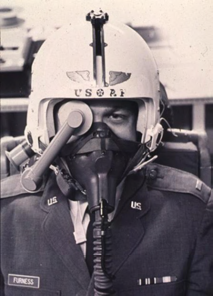
\includegraphics[width=\textwidth]{image/airforce1}
		\caption{دوربین نصب شده بر روی سر یک خلبان}
		\label{fig:gull}
	\end{subfigure}
	~ %add desired spacing between images, e. g. ~, \quad, \qquad, \hfill etc. 
	%(or a blank line to force the subfigure onto a new line)
	\begin{subfigure}[b]{0.5\textwidth}
		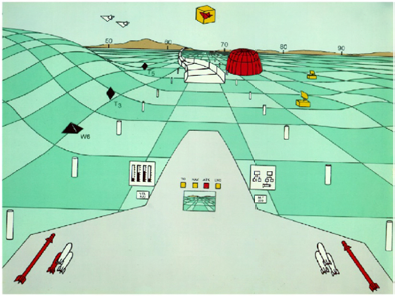
\includegraphics[width=\textwidth]{image/airforce2}
		\caption{تصویر شبیه سازی شده در پروژه}
		\label{fig:tiger}
	\end{subfigure}
	~ %add desired spacing between images, e. g. ~, \quad, \qquad, \hfill etc. 
	%(or a blank line to force the subfigure onto a new line)
	
	\caption{پروژه Super-Cockpit \cite{Furness2}}\label{fig:Super-Cockpit}
\end{figure}


در سال ۱۹۸۱ آژانس ملی فضا و هواشناسی \lr{(NASA)} شروع به تحقیق بر روی این فنّاوری نمود و کلاه و نمایشگر مخصوص به خود را نیز طراحی کرد که می‌توانست برای آموزش فضانوردان با ایجاد تصاویر مجازی کمک بکند\cite{Furness2}.
\\
\section{انگیزه پژوهش}
\noindent
گارتنر\LTRfootnote{Gartner}، شرکت پژوهشی و مشاوره آمریکایی است، که درزمینه ارائه خدمات برون‌سپاری، تحقیق و پژوهش و مشاوره فناوری اطلاعات فعالیت می‌نماید. شرکت گارتنر در سال ۱۹۷۹ توسط Gideon Gartner راه‌اندازی شد و در حال حاضر دارای عملیات در ۸۵ کشور جهان است. دفتر مرکزی این شرکت در شهر استنفورد، کنتیکت، ایالات‌متحده آمریکا قرار دارد و سهام آن در بازار بورس نیویورک معامله می‌شود\LTRfootnote{https://en.wikipedia.org/wiki/Gartner}.
\\
این شرکت هرساله نموداری را معرفی می‌کند که در آن به معرفی تکنولوژی‌های روز پرداخته و موقعیت آنها آن‌ها را بررسی می‌کند\LTRfootnote{https://www.gartner.com/smarterwithgartner/5-trends-emerge-in-gartner-hype-cycle-for-emerging-technologies-2018/}.شکل:\ref{fig:gartner}
\\

\begin{figure}[tb]
	\centering
	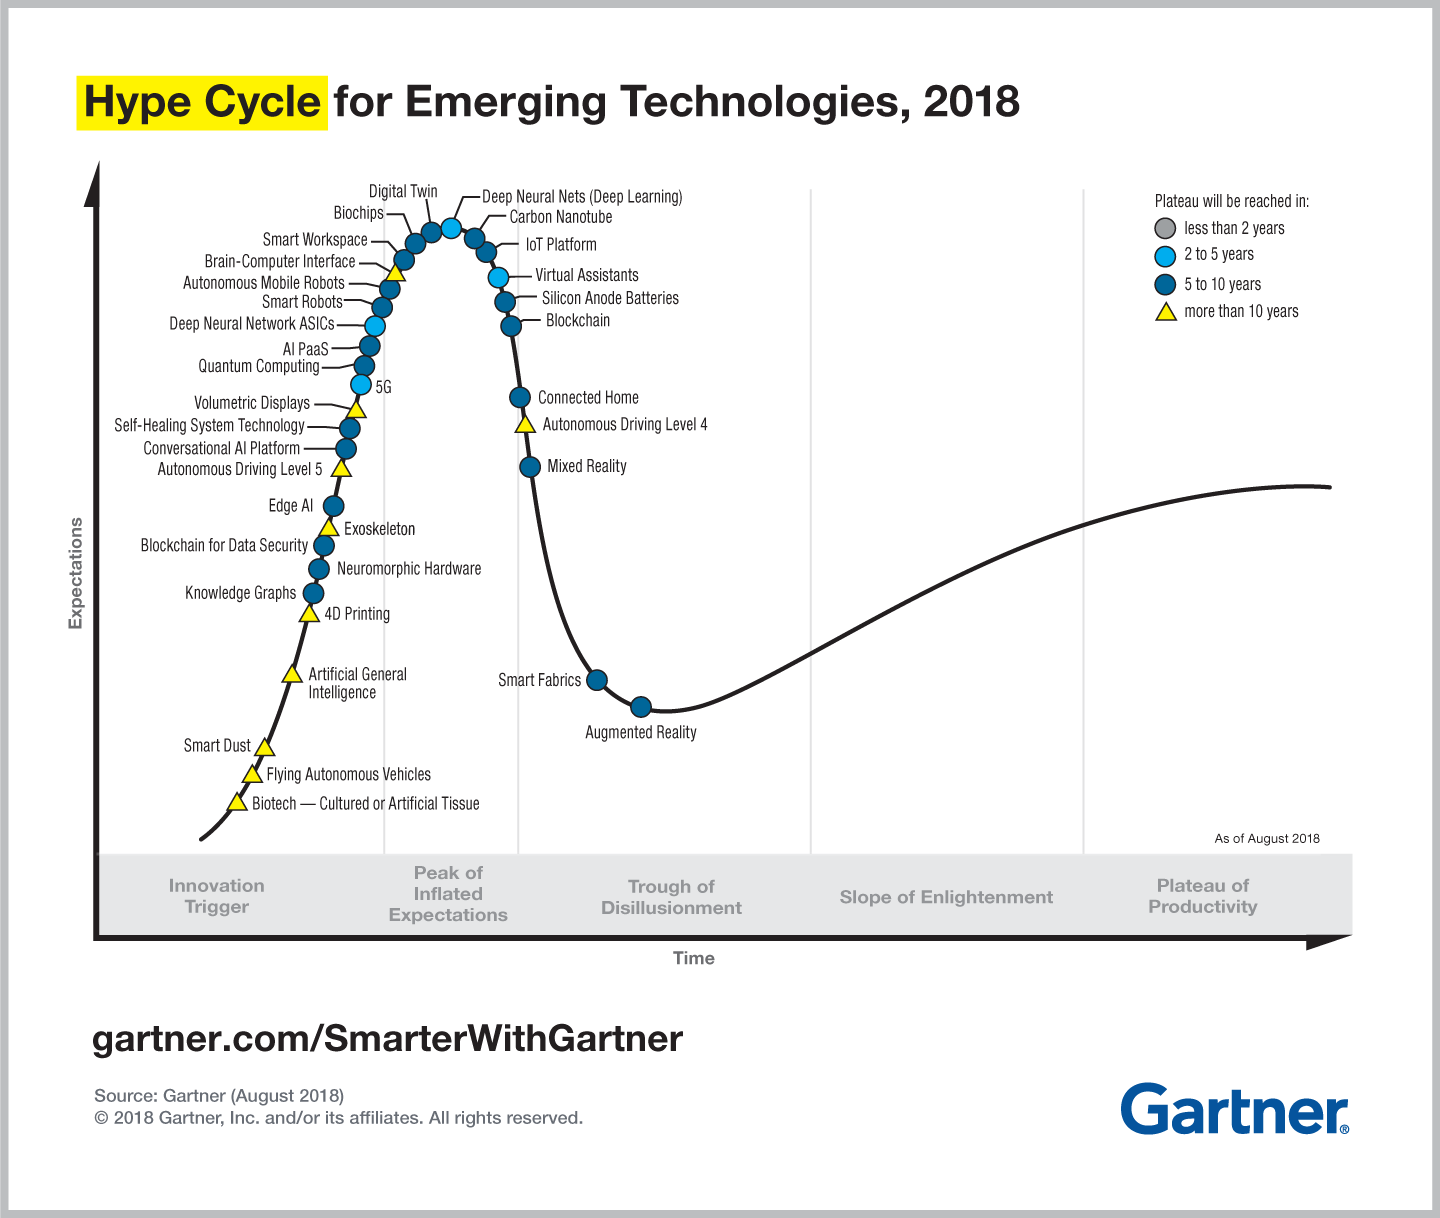
\includegraphics[width=1\linewidth]{image/gartner}
	\caption {نمودار موقعیت فنّاوری‌ها در سال ۲۰۱۸}
	\label{fig:gartner}
\end{figure}
\noindent
این نمودار از ۵ قسمت مختلف تشکیل‌شده است: 
\\
\textbf{
	۱-راه افتادن فنّاوری \LTRfootnote{Technology Trigger} : }در این مرحله یک فنّاوری مفهوم‌سازی می‌شود، پتانسیل‌های آن موردبررسی قرار می‌گیرد و شروع به اثبات ادعاهای خود می‌کند.
\\
\textbf{
	۲-اوج انتظارات \LTRfootnote{Peak of Inflated Expectations} : }در این مرحله تکنولوژی به پیاده‌سازی می‌رسد و نظریات و تبلیغات در رابطه با موفقیت‌آمیز بودن و یا نبودن آن مطرح می‌شود.
\\
\textbf{
	۳-مرحله سرخوردگی \LTRfootnote{Trough of Disillusionment} :} در این مرحله مشکلات تکنولوژی نمایان می‌شود و شروع تلاش‌ها برای رفع این مشکلات است.
\\
\textbf{
	۴-شیب روشنگری \LTRfootnote{Slope of Enlightenment} :} در این مرحله شرکت‌های مختلف به این تکنولوژی روی می‌آورند و پتانسیل‌های این فنّاوری برای آینده نمایان‌تر می‌شود.
\\
\textbf{
	۵-فلات بهره‌وری \LTRfootnote{Plateau of Productivity} :} در اینجا استفاده از این فناوری گسترده و همه‌گیر شده و تعداد خیلی زیادی از شرکت‌های کوچک و بزرگ به آن روی می‌آورند.
\\
همان‌طور که ملاحظه می‌شود این فنّاوری در مرحله سوم قرار دارد و مشکلاتی دارد که باعث می‌شود زمینه خوبی برای مطالعه و تحقیق باشد و همچنین بسیار گرایش برای آن وجود دارد به‌طوری‌که شرکت بزرگی مانند Gartner این فنّاوری را پیشنهاد می‌دهد و پیش‌بینی می‌کند که یکی از فنّاوری‌هایی باشد که در آینده نزدیک شاهد ظهور و گسترده شدن آن خواهیم بود.
\\
یکی از مراجع مهم و معروف برای مقاله‌ها در این زمینه، نشست بین‌المللی واقعیت افزوده و واقعیت ترکیبی \lr{(ISMAR)}\LTRfootnote{International Symposium on Mixed and Augmented Reality (ISMAR)} است که در قالب \lr{IEEE Computer Society } به‌صورت سالیانه برگزار می‌شود، با بررسی و ارزیابی ۲ دهه از مقاله‌های منتشرشده در این کنفرانس، به نمودارهای زیر می‌رسیم.‌\RTLfootnote{در این مقاله منظور از \lr{Rendering} نحوه پردازش تصویر است و با واژه رندرینگ در این تحقیق متفاوت است. }\cite{ismar}.
\begin{figure}
	\centering
	\begin{subfigure}[b]{1\textwidth}
		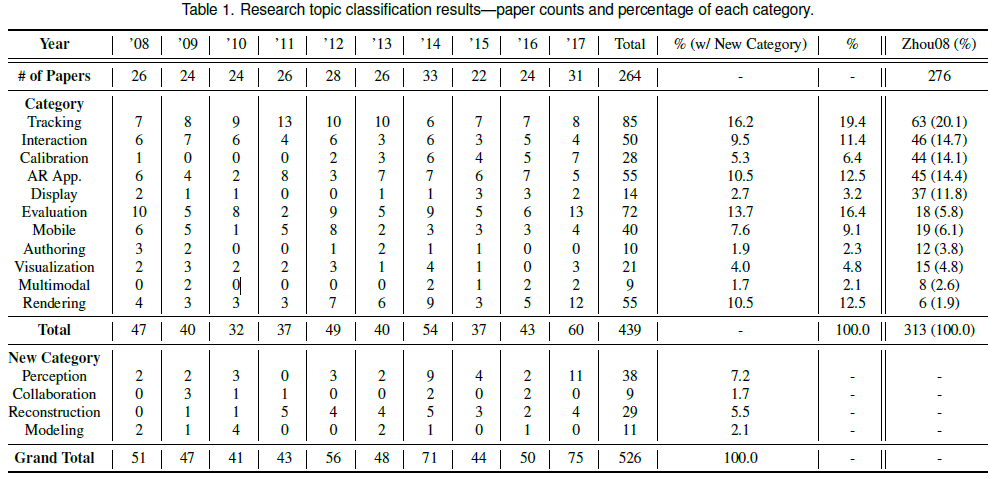
\includegraphics[width=\textwidth]{image/ismar1}
		\caption{تعداد مقاله ها بر اساس موضوع}
		\label{fig:gull}
	\end{subfigure}
	~ %add desired spacing between images, e. g. ~, \quad, \qquad, \hfill etc. 
	%(or a blank line to force the subfigure onto a new line)
	\begin{subfigure}[b]{0.4\textwidth}
		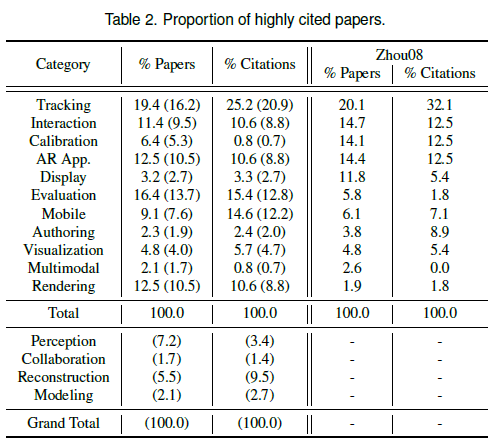
\includegraphics[width=\textwidth]{image/ismar2}
		\caption{ارجاع به مقالات به نسبت تعداد}
		\label{fig:tiger}
	\end{subfigure}
	~ %add desired spacing between images, e. g. ~, \quad, \qquad, \hfill etc. 
	%(or a blank line to force the subfigure onto a new line)
	\begin{subfigure}[b]{0.5\textwidth}
		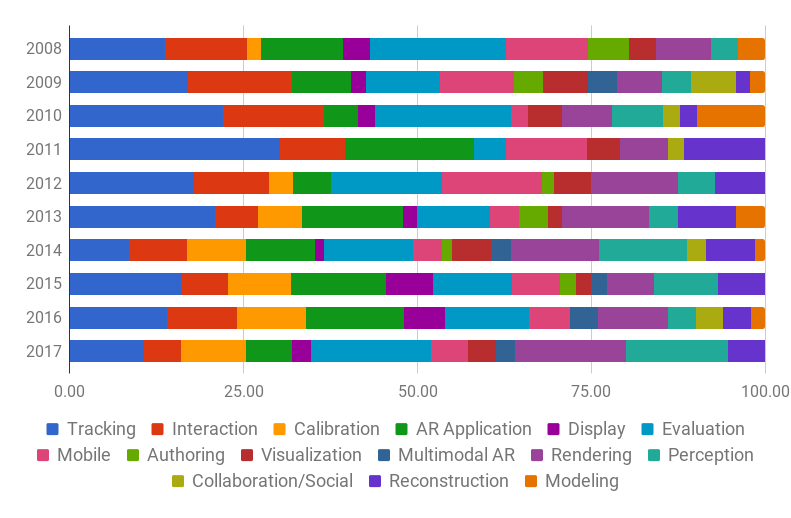
\includegraphics[width=\textwidth]{image/ismar3}
		\caption{مقابسه تمایل نویسندگان بر اساس موضوع}
		\label{fig:tiger}
	\end{subfigure}
\begin{subfigure}[b]{0.5\textwidth}
	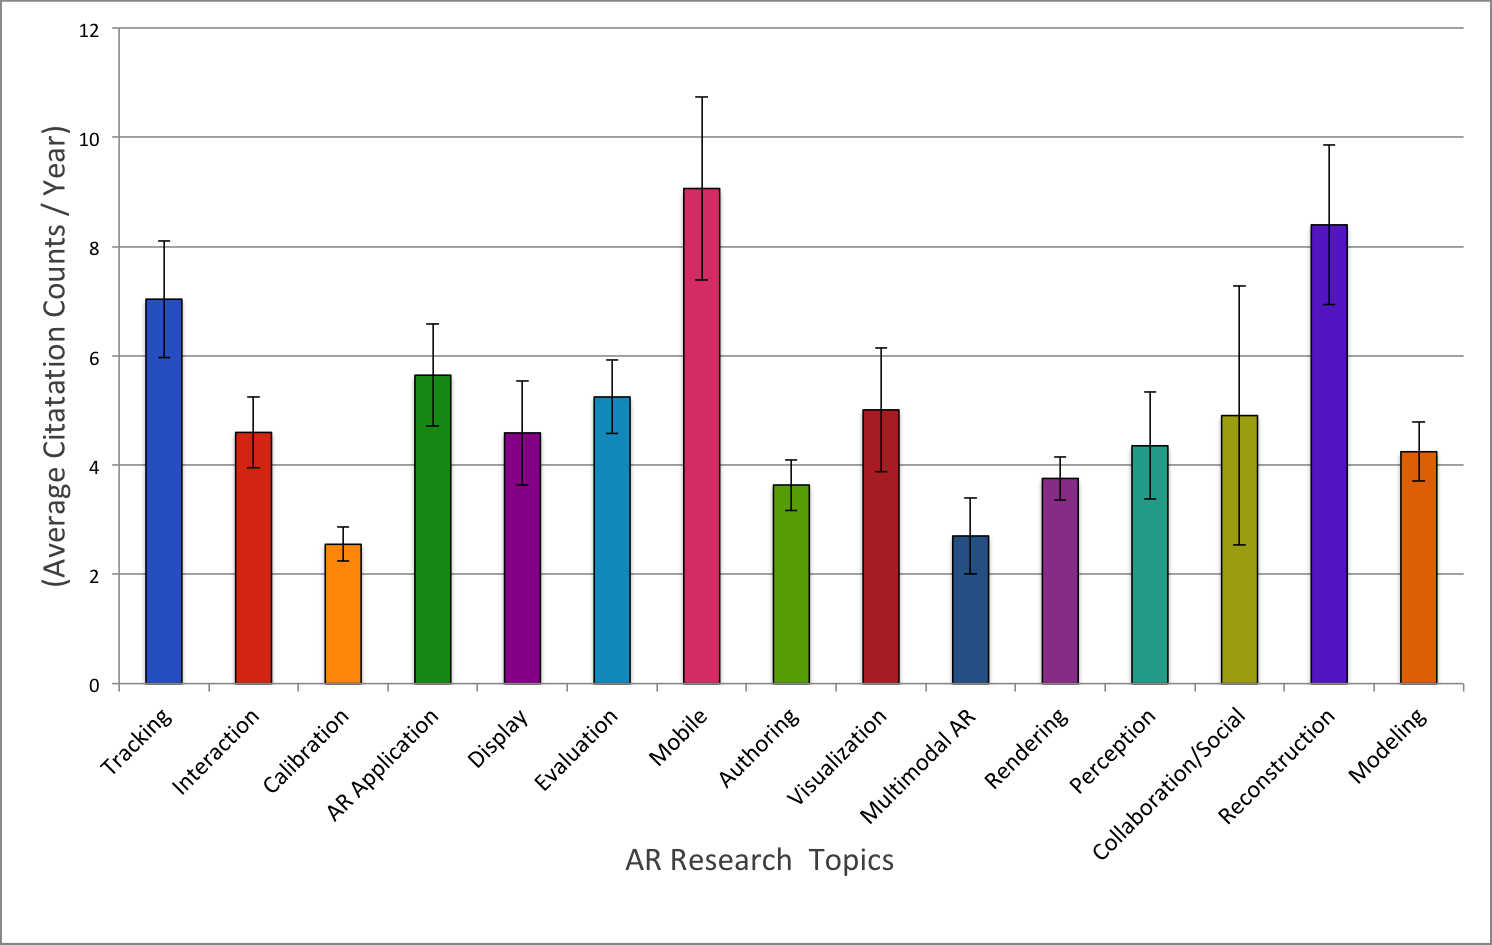
\includegraphics[width=\textwidth]{image/ismar4}
	\caption{میانگین ارجاع به مقالات در سال بر اساس موضوع}
	\label{fig:tiger}
\end{subfigure}
	\caption{بررسی 2 دهه کنفرانس ISMAR\cite{ismar}}\label{fig:ISMAR}
\end{figure}

 همان‌طور که از نتایج پیدا است یکی از حوزه‌های موردعلاقه محققین ردیابی\LTRfootnote{Tracking}، است که مقاله‌های زیادی در این حوزه منتشر می‌شود و همچنین ارجاعات به این مقالات نیز بالا می‌باشد.



\section{بیان ساختار فصل‌های بعدی}
بخش‌بندی سمینار به شکل زیر است:
\\
\textbf{
	بخش دوم:} در این بخش درخت موضوعی را به نمایش می‌گزاریم، ادبیات موضوع را مطرح کرده، کلیه اطلاعات لازم در واقعیت افزوده را شرح داده و به بیان حوزه‌های مختلف در آن می‌پردازیم و به‌اختصار آن‌ها را شرح می‌دهیم.
\\
\textbf{
	بخش سوم: } در این بخش به معرفی رندرینگ در واقعیت افزوده می‌پردازیم و اجزای آن را شرح می‌دهیم و سپس تمرکز خودمان را بر روی ردیابی (Tracking) می‌گزاریم و روش‌های مختلف درون آن را شرح می‌دهیم و کارهای گذشته را ذکر می‌کنیم.
\\
\textbf{
	فصل چهارم:} در این فصل روش‌های مختلف را باهم مقایسه کرده و مسئله‌ای را مطرح کرده و به چالش‌های آن می‌پردازیم.
\\
\textbf{
	فصل پنجم:} در این فصل به نتیجه‌گیری کلی می‌پردازیم.

\cchapter{ادبیات تحقیق}
\section{معرفی}
\subsection{انواع رابط کاربری}
\noindent
محقق \lr{Ron Azuma} بیان می‌کند که واقعیت افزوده باید شامل ۳ ویژگی باشد\cite{Azuma}:
\\
۱- باید توانایی ترکیب دنیای واقعی و مجازی را دارا باشد.
\\
۲- باید با دنیای واقعی در ارتباط باشد.
\\
۳- باید به‌صورت ۳ بعدی قابل استناد باشد.
\\
مثال شبکه خبری \lr{CNN} هر سه این شرایط را دارا می‌باشد. تصویر مجازی خبرنگار \lr{Jessica Yellin} به‌صورت زنده بر روی صحنه ظاهر شد و همچنین توانایی برقراری ارتباط و صحبت با خبرنگار \lr{Wolf Blitzer} در همان زمان بود و تصویر مجازی به‌صورت سه بعدی قابل‌نمایش بود.
\\
در یک سیستم واقعیت افزوده هر سه شرط باید رعایت شود و همچنین باید شامل یک سیستم کامپیوتری که قادر است تصاویر مجازی تولید کند و به دنیای واقعی اضافه کند باشد، همچنین باید یک سیستم ردیابی \LTRfootnote{Tracking} را دارا باشد تا بتواند نقطه مناسب برای ظاهر شدن تصویر مجازی را شناسایی بکند و تصویر مجازی را بر روی آن به نمایش درآورد. در قسمت بعدی این تحقیق مفصل به بیان سیستم ردیابی می‌پردازیم.
\\
باید توجه شود که در تعریف \lr{Azuma} هیچ محدودیتی آورده نشده در مورد نوع تکنولوژی که برای ظاهر کردن تصاویر در دنیای واقعی از آن استفاده می‌کنیم، همچنین در سیستم لزومی به‌ظاهر شدن تصویر نمی‌باشد و می‌تواند به پخش موسیقی و یا پخش فیلم بپردازد.
\\
اگر با یک دید جامع نگاه بکنیم، واقعیت افزوده آخرین تلاش توسط محققین و مهندسین برای حذف رابط کاربری در کامپیوترها و افزایش تعامل کاربر با دنیای واقعی است.\lr{Rekimoto}  تفاوت بین رابط‌های میز کار سنتی \LTRfootnote{traditional desktop computer interfaces} با تلاش‌هایی که در جهت حذف رابط کاربری انجام‌شده است را متمایز ساخت\cite{Rekimoto}. همان‌طور که در شکل \ref{fig:Rekimoto} قابل‌مشاهده است، \lr{Rekimoto} به معرفی انواع رابط‌های کاربری پرداخت و ۴ مدل را معرفی نمود.
\\
\begin{figure}[tb]
	\centering
	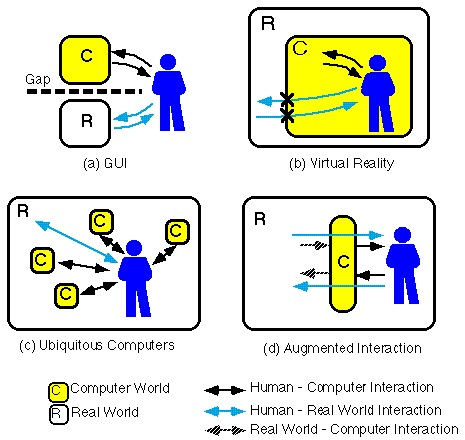
\includegraphics[width=1\linewidth]{image/style}
	\caption {انواع رابط‌های کاربری\cite{Rekimoto}}
	\label{fig:Rekimoto}
\end{figure}
\textbf{1- مدل رابط گرافیکی کاربر \lr{(GUI)}:\LTRfootnote{graphical user interface}}در این مدل کاربر با استفاده از اشکال گرافیکی که توسط کامپیوتر در اختیارش قرار می‌گیرد ارتباط برقرار می‌کند مانند آیکون‌ها، محیط ویندوز، منوها و ...
\\
\textbf{
	۲- مدل واقعیت مجازی:\LTRfootnote{Virtual Reality} }در این مدل کاربر با استفاده از کلاهی که بر روی سر و چشمانش قرار می‌گیرد وارد دنیای مجازی شده و درون این دنیا قرار می‌گیرد و با استفاده از دستکش‌ها و یا دسته‌های مخصوص شروع به تعامل با دنیای مجازی می‌کند و به‌اصطلاح درون این دنیا غواصی\LTRfootnote{immersive} می‌کند و از دنیای واقعی جدا می‌شود.
\\
\textbf{۳ -مدل پردازش همه‌جا حاضر:\LTRfootnote{Ubiquitous Computing} }در این مدل سنسورها و پردازشگرها در دنیای واقعی جاسازی‌شده‌اند.
\\
\textbf{
	۴- واقعیت افزوده:\LTRfootnote{Augmented Reality}} مشکل مدل دوم (واقعیت مجازی) این است که کاربر از دنیای واقعی جداشده و توانایی ارتباط با آن را ندارد ولی در این مدل کاربر علاوه بر توانایی تعامل با دنیای مجازی، قادر است با دنیای واقعی نیز تعامل بکند و این دو نه‌تنها مشکلی برای هم ایجاد نمی‌کنند، بلکه مکمل و کمک‌کننده به یکدیگر هستند.
\\
همان‌طور که در تعاریف بالا می‌توانیم ببینم، رابطه نزدیکی بین واقعیت مجازی و واقعیت افزوده وجود دارد، همچنین هر دو آن‌ها دارای صفحه‌نمایشی که بر روی سر نصب‌شده\LTRfootnote{head mounted displays}، سیستم ردیابی و دستگاه‌های ورودی دستی\LTRfootnote{handheld input devices} می‌باشند، بااین‌حال بین این دو تفاوت‌های مهمی وجود دارد.
\\
هدف اصلی از واقعیت مجازی، استفاده از تکنولوژی برای جایگزینی آن با دنیای واقعی است و در مقابل آن در واقعیت افزوده، تکنولوژی سعی بر آن دارد  با استفاده از محتوای دیجیتال\LTRfootnote{digital content} بدون آنکه به کاربر حس غوطه‌ور شدگی دست بدهد به دنیای واقعی بیفزاید. در واقعیت مجازی دستگاه نمایشگر باید کاملاً جامع باشد و میدان گسترده‌ای از دید را پوشش بدهد و گرافیک‌های ۳ بعدی تا حد امکان واقعی به نظر بیایند. ازآنجاکه کاربر به مدت زیادی قادر به دیدن دنیای واقعی نمی‌باشد، در واقعیت مجازی سیستم ردیابی نیاز به دقیق بودن به نسبت دنیای واقعی را ندارد و این حساسیت در آن کمتر می‌باشد.
\\
در مقابل، در  واقعیت افزوده، سیستم نمایش می‌تواند به‌صورت غیر غوطه‌ور کننده، با گستردگی دید کم و با استفاده از گرافیک‌های کوچک باشد. ولی در اینجا، سیستم ردیابی باید بسیار دقیق باشد و توانایی داشته باشد تا محتوای مجازی را دقیقاً بر روی دنیای واقعی قرار بدهد. برای کاربران واقعیت افزوده بسیار ساده است تا متوجه چندین میلی‌متر تفاوت قرار گرفتن محتوای مجازی با دنیای واقعی بشوند.
\\
\subsection{واقعیت ترکیبی}
برای توضیح بیشتر برای واقعیت افزوده می‌توانیم به نتیجه تحقیق Milgram و Kishino نگاهی بیندازیم\cite{Milgram}. آنها مفهومی با نام واقعیت ترکیبی\LTRfootnote{Mixed Reality} را معرفی نمودند که این مفهوم دو مفهوم واقعیت و مجازی را با یکدیگر ترکیب می‌کند و همچنین طبقه‌بندی‌هایی را بر اساس میزان ترکیب مجازی و واقعیت بیان می‌کند. در سمت راست محیط مجازی\LTRfootnote{Virtual Environment} را می‌بینیم، جایی که دید کاربر از جهان توسط کامپیوترهایی که تصاویر مجازی تولید می‌کنند کاملاً جایگزین شده است. در سمت مخالف، یعنی در سمت چپ ما شاهد محیط واقعی\LTRfootnote{Real Environment} هستیم که در آن کاربر هیچ‌گونه دید و درکی از عناصر مجازی ندارد و کاملاً درون دنیای واقعی قرارگرفته است. هر چه از محیط واقعی به سمت محیط مجازی حرکت کنیم، میزان عناصر مجازی در دید کاربر افزایش میابد و این محیط مابین، به دو دسته دیگر تقسیم می‌شوند. دسته واقعیت افزوده که در آن میزان واقعیت در دید کاربر خیلی بیشتر از مجازی است و دسته مجازی افزوده‌شده\LTRfootnote{Augmented Virtuality} که درون آن، بیشتر دید کاربر را عناصر مجازی تشکیل داده است و قسمت کمی را عناصر واقعی تشکیل می‌دهند.
\\
با استفاده از شکل \ref{fig:Mixed}، به این نتیجه می‌رسیم که واقعیت افزوده خود به‌تنهایی به‌عنوان دسته مجزا شناخته نمی‌شود بلکه بخشی از هر دو را تشکیل می‌دهد.

\begin{figure}[!ht]
	\centering
	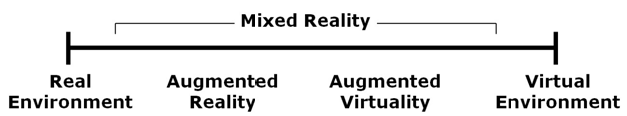
\includegraphics[width=1\linewidth]{image/mixedreality}
	\caption {شکل معرفی شده برای Reality Mixed توسط Milgram\cite{Milgram}}
	\label{fig:Mixed}
\end{figure}

\section{انواع دستگاه‌های واقعیت افزوده}
دستگاه‌های نمایشگری که با استفاده از آن‌ها تکنولوژی واقعیت افزوده را به نمایش درمی‌آوریم به سه دسته کلی تقسیم می‌شوند\cite{Julie}:
\\
\subsection{
	۱- نمایشگرهایی که بر روی سر نصب می‌شوند\protect\LTRfootnote{head mounted displays
		(HMD)} }این نوع از نمایشگرها بر روی سر قرار می‌گیرند مانند کلاه ایمنی و یا مانند عینک، در جلوی چشمان قرار داده می‌شوند و  قادر هستند هر دو تصویر از دنیای مجازی و واقعی را بر روی‌هم قرار داده و به کاربر نشان بدهند شکل. این دستگاه‌ها به دو صورت کار می‌کنند.
\begin{itemize}
	\item \textbf{1- دیدن از طریق ویدیو\LTRfootnote{Video-see-through}:} در این مدل، نیاز داریم تا کاربر، ۲ دوربین را بر روی سرخود قرار دهد و با استفاده از پردازش‌های تصاویر این دو دوربین، تصاویر ۳ بعدی از محیط را  به‌صورت زنده دریافت کنیم و همزمان با استفاده از یک کامپیوتر، تصاویر ۳ بعدی مجازی را طراحی بکنیم و با تصاویر دریافتی از دوربین‌ها، ادغام بکنیم، در این روش به دو مشکل برخورد می‌کنیم، مشکل اول کیفیت تصاویر است که وابسته به‌وضوح \LTRfootnote{resolution} دوربین‌ها و پردازشگرهای تصاویر است و همچنین وابسته به کیفیت تصویر تولیدشده توسط کامپیوتر است و مشکل بعدی این است که باید سرعت کارها در این نوع بالا باشد تا تأخیر \LTRfootnote{latency}دریافت تصاویر و پردازش و سپس نمایش را به حداقل برسانیم.
	\item \textbf{
		2- دیدن از طریق نور:\LTRfootnote{optical-see-through} }در این مدل کاربر با استفاده از لنزها، قادر است دنیای واقعی را ببیند، و با استفاده از دستگاه‌های خاص و تابش نور به لنزها، تصاویر ۳ بعدی را برای کاربر طراحی می‌کنیم. در اینجا کیفیت تصاویر دریافتی به نسبت روش قبل بالاتر است زیرا برای دیدن دنیای واقعی نیازی به‌وضوح نمایشگر نداریم ولی برای ایجاد کردن تصاویر ۳ بعدی در این روش مشکل است. همچنین به دلیل اینکه تصاویر محیط واقعی را بدون واسطه دریافت می‌کنیم، تأخیر در اینجا نیز کمتر از روش قبلی است.
\end{itemize}

\begin{figure}[tb]
	\centering
	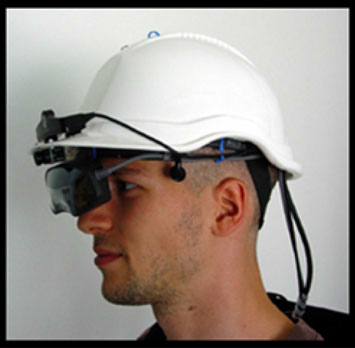
\includegraphics[width=0.6\linewidth]{image/hmd}
	\caption {نمونه‌ای از نمایشگرهای نصب‌شده بر روی سر\cite{Julie}}
	\label{fig:hmd}
\end{figure}

\subsection{نمایشگرهای دستی\protect\LTRfootnote{Handheld displays} :}
این نوع از نمایشگرها، با کمک گرفتن از دستگاه‌های محاسباتی کوچک که دارای نمایشگر می‌باشند کار می‌کنند و برای ادغام کردن تصاویر مجازی با دنیای واقعی از روش "دیدن از طریق ویدئو" استفاده می‌کنند. به‌عنوان‌مثال برای این نوع از نمایشگرها می‌توان تلفن‌های  همراه هوشمند را مثال زد که علاوه بر دارا بودن ویژگی‌های ذکرشده، دارای سنسورهایی مانند "سیستم موقعیت یاب جهانی"\LTRfootnote{Global Positioning System (GPS)} و قطب نمای دیجیتال هستند که برای ردیابی می‌توان از آن‌ها استفاده نمود
\begin{figure}[tb]
	\centering
	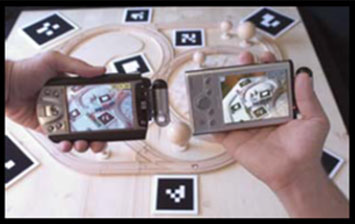
\includegraphics[width=0.7\linewidth]{image/mobile}
	\caption {نمونه‌ای از نمایشگرهای دستی\cite{Julie}}
	\label{fig:mobile}
\end{figure}
\subsection{نمایشگرهای فضایی\protect\LTRfootnote{spatial displays}}
در این نوع از نمایشگرها ما شاهد واقعیت افزوده فضایی\LTRfootnote{Spatial Augmented Reality (SAR)} هستیم که با استفاده از ویدئو پروژکتور، عناصر نوری، هولوگرام‌ها و برچسب‌های فرکانس رادیویی به‌صورت مستیم عناصر مجازی را به درون دنیای واقعی میاورند و دیگر کاربر نیازی ندارد که دستگاهی را بر روی سرخود قرار بدهد و یا اینکه دستگاهی را حمل بکند شکل\ref{fig:sar}. در نمایشگرهای فضایی، بیشتر فنّاوری بدون وابستگی به کاربر است و بدون دخالت او، عناصر مجازی را با روش اضافه کردن مستقیم\LTRfootnote{direct
	augmentation} با دنیای واقعی ادغام می‌کنیم\cite{Bimber}.
\begin{figure}[tb]
	\centering
	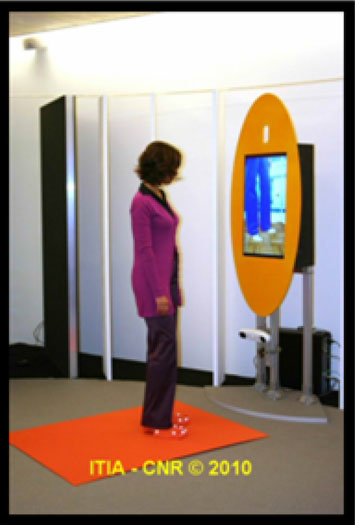
\includegraphics[width=0.6\linewidth]{image/sar}
	\caption {نمونه‌ای از نمایشگرهای فضایی\cite{Bimber}}
	\label{fig:sar}
\end{figure}
\section{ورودی و تعامل}
سیستم‌های واقعیت افزوده می‌توانند روش‌های مختلف دریافت ورودی را با یک دیگر ترکیب بکنند، مانند دریافت از صوت، دستکش‌های مخصوص، لمس کردن تصویر، پردازش تصویر و غیره. دریافت ورودی‌ها در برنامه‌های مختلف با توجه به نیاز هر برنامه متفاوت است.
سیستم‌های طراحی‌شده برای دریافت ورودی و تعامل با واقعیت افزوده را می‌توان به ۵ دسته زیر تقسیم نمود:

\subsection{مرورگرهای اطلاعات\protect\LTRfootnote{Information Browsers}: }رابطی است برای نشان دادن اطلاعات واقعیت افزوده بر روی دنیای واقعی. این نوع از دریافت اطلاعات و تعامل، نماینده‌ای از برنامه‌های واقعیت‌های افزوده است و درجایی کار می‌کنند که نمایشگر واقعیت افزوده به‌عنوان پنجره‌ای به‌سوی فضای اطلاعاتی در نظر گرفته می‌شود و وظیفه اصلی کاربر این است که این پنجره را کنترل کرده تا بتواند اطلاعات را دریافت بکند. اولین نمونه از این برنامه NaviCam شکل \ref{fig:Rekimoto} است که بر روی گوشی‌های هوشمند پیاده‌سازی شد. این نوع از برنامه‌ها نیاز به انجام تعامل‌های پایه دارد و شیوه کار آن‌ها به این صورت است که صحنه واقعیت افزوده را پردازش می‌کنند و اطلاعات برای کاربر پردازش می‌شود \cite{Rekimoto}.
\begin{figure}[tb]
	\centering
	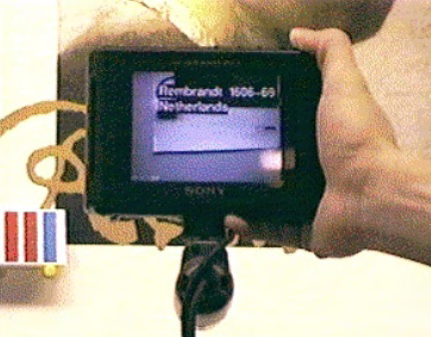
\includegraphics[width=0.6\linewidth]{image/navicam}
	\caption {نمونه‌ای از پروژه NaviCam\cite{Rekimoto}}
	\label{fig:Rekimoto}
\end{figure}
\subsection{رابط کاربر ۳ بعدی\protect\LTRfootnote{3D User Interfaces}:}
در این مدل با استفاده از تکنیک‌های تعاملی ۳ بعدی به ارتباط با محتوا در فضا می‌پردازیم. این روش یکی از راه‌های جذاب و مناسب برای تعامل است. Bowman به‌طور خلاصه این فرایند را به سه قسمت تقسیم کرده است\cite{Bowman}.
\begin{itemize}
	\item 
	\textbf{
		جهت‌یابی\protect\LTRfootnote{navigation}: }در این قسمت نیاز است که عنصر ۳ بعدی دیده شود و در اصل به سمت آن جهت‌یابی شویم، این قسمت بسیار ساده است و با حرکات بدن کاربر قابل پیاده‌سازی است. در بسیاری از دستگاه‌ها کاربر می‌تواند در سه بعد حرکت کند و در هر سه جهت نیز بچرخد.
	\item 
	\textbf{
		انتخاب\LTRfootnote{selection}:} در این قسمت نیاز است تا کاربر بتواند برای تعامل، عنصر مجازی را انتخاب بکند، برای این قسمت می‌توان از دستگاه‌های مختلف مانند سنسورها، جوی استیک\LTRfootnote{joysticks} و... استفاده کرد.
	\item 
	\textbf{
		دست‌کاری\LTRfootnote{manipulation}:} این قسمت گام آخر است و کاربر می‌تواند تعامل خود را با عناصر مجازی به‌راحتی انجام دهد.
\end{itemize}
\begin{figure}[tb]
	\centering
	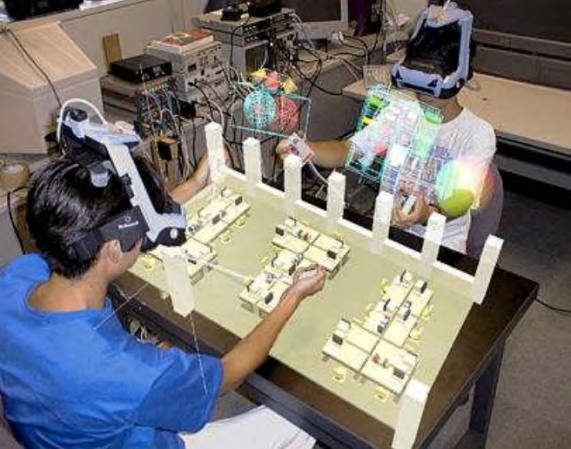
\includegraphics[width=0.6\linewidth]{image/3d}
	\caption {استفاده از رابط کاربر ۳ بعدی \cite{Bowman}}
	\label{fig:Bowman}
\end{figure}
\subsection{رابط کاربر قابل‌ لمس\protect\LTRfootnote{Tangible User Interfaces} :}
در این نوع از رابط‌ها، برای ارتباط با عناصر مجازی از عناصر دنیای واقعی استفاده می‌کنیم. این اجسام مانند پلی بین دنیای واقعی و دنیای مجازی می‌باشند و تعامل را برقرار می‌سازند. این روش یکی از روش‌های نوین برای تعامل با دنیای مجازی است، اما مشکلات خود را نیز دارا است، به‌عنوان‌مثال، وقتی‌که قصد داریم یک عنصر مجازی را بر روی عنصر فیزیکی به وجود بیاوریم، این عنصر مجازی یا باید با استفاده از پرتو تابیده شود، و یا بر روی نمایشگر کاربر ظاهر شود، در این رابط، ممکن است فاصله‌ای بین جسم مجازی و فیزیکی به وجود بیاید که ناخوشایند است\cite{Kato}.
\begin{figure}[tb]
	\centering
	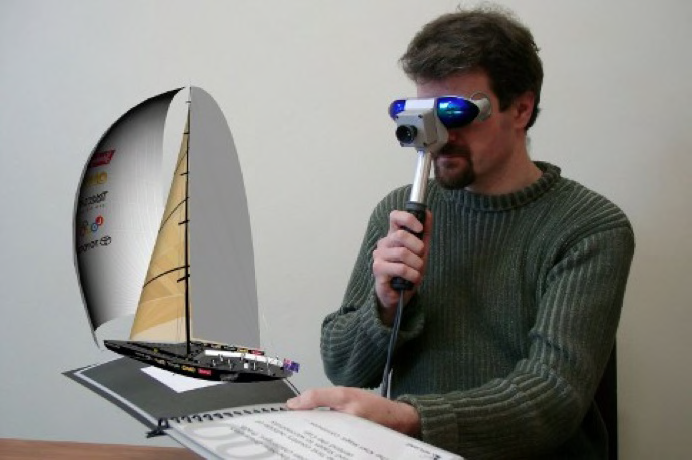
\includegraphics[width=0.6\linewidth]{image/tar}
	\caption {استفاده از رابط کاربر قابل لمس \cite{Kato}}
	\label{fig:Bowman}
\end{figure}
\subsection{رابط کاربر طبیعی \protect\LTRfootnote{Natural User Interfaces} :}
در این مدل از اجزای طبیعی بدن مانند دست‌ها استفاده می‌کنیم، در این حالت اجزای بدن می‌توانند ردیابی شوند و تشخیص داده شوند با استفاده از سنسورهای مختلفی که کاربر می‌تواند پوشیده باشد. سنسورهای مختلفی در اندازه‌ها و شکل‌های مختلفی برای این کار ساخته‌شده‌اند.
با پیشرفت کامپیوترها، سیستم‌های واقعیت افزوده توانستند حرکت و ژست بدن کاربر را بدون نیاز به سنسورها تشخیص بدهند. به‌طور مثال Lee توانست سیستمی را طراحی کند که توانایی شناسایی دست و حرکت‌های آن را داشته باشد\cite{Lee}.
\begin{figure}[!ht]
	\centering
	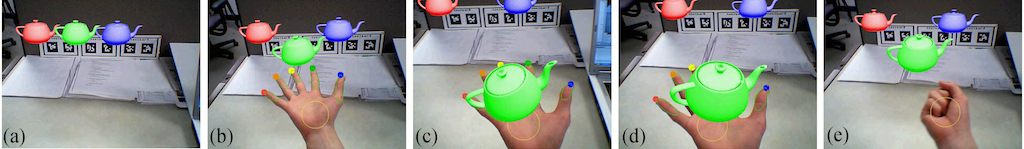
\includegraphics[width=1\linewidth]{image/handyar}
	\caption {استفاده از رابط کاربر طبیعی \cite{Lee}}
	\label{fig:Bowman}
\end{figure}

\subsection{رابط چند منظوره\protect\LTRfootnote{Multimodal Interfaces} :}
برای تعامل قوی‌تر در برنامه‌های واقعیت افزوده، محققین سعی کردند تا مدل‌های مختلفی از ورودی‌ها را با یکدیگر ترکیب کنند، در این میان ترکیب گفتار\LTRfootnote{speech} و تشخیص ژست\LTRfootnote{gesture recognition}، یکی از گسترده‌ترین و فعال‌ترین بخش‌ها بوده است.
\\
Lee در این رابطه تحقیقات زیادی انجام داد و یک سیستم چندمنظوره را طراحی کرد که در آن با استفاده از یک دوربین به  ردیابی ژست دست می‌پرداخت و همچنین با دریافت گفتار و ترکیب این دو، دستورات را شناسایی می‌کرد و به تعامل با کامپیوتر می‌پرداخت.
او توانست دقت را در این روش شناسایی کند و بیان کرد که با این ترکیب در سیستم واقعیت افزوده ۲۵ درصد سریع‌تر به نسبت تشخیص ژست به‌تنهایی، می‌توان به تعامل پرداخت\cite{Lee2}.
\begin{figure}[!ht]
	\centering
	\begin{subfigure}[b]{0.5\textwidth}
		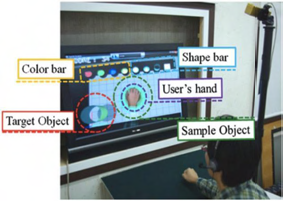
\includegraphics[width=\textwidth]{image/lee2}
		
		
	\end{subfigure}
	~ %add desired spacing between images, e. g. ~, \quad, \qquad, \hfill etc. 
	%(or a blank line to force the subfigure onto a new line)
	\begin{subfigure}[b]{0.4\textwidth}
		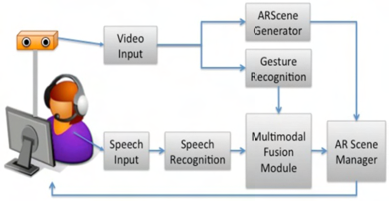
\includegraphics[width=\textwidth]{image/lee1}
		
	\end{subfigure}
	\caption{رابط چند منظوره\cite{Lee2}}\label{fig:lee2}
\end{figure}